We experimented with the RNN-GSN described by Algorithm \ref{algo} on sequences of MNIST images and standard MIDI datasets.

Each RNN-GSN was first initialized with GSN parameters and trained with noise scheduling, which has been shown to help the network learn appropriate features during stochastic gradient descent \cite{noise_schedule}.

The GSNs used $1500$ hidden units, $3$ hidden layers, and $5$ walkbacks, and the RNNs used $1500$ hidden units and $1$ hidden layer. $Tanh$ activation was used for hidden units, $sigmoid$ activation for visible inputs, and the network was trained using stochastic gradient descent on a binary cross-entropy cost with momentum of $0.5$ on the parameters and annealing of $0.995$ on the learning rate starting at $0.25$. GSN noise was added as salt-and-pepper, starting at $0.7$ with a schedule rate of $0.98$. MNIST input dimensionality is 784 and MIDI input dimensionality is 88.
\subsection{Sequences of MNIST digits}
The MNIST dataset is a series of greyscale handwritten digits. To introduce a temporal structure, we created three increasingly complex sequences of images. Log-likelihoods are estimated by a Parzen density estimator, which is biased. Further validation can be seen qualitatively by the predicted samples produced from the models.

\textbf{Sequence1} is a simple linear sequence of digits \{0,1,2,3,4,5,6,7,8,9,...\} repeating. As seen with the TGSN example in Figure \ref{fig:tgsn}, this sequence can be modeled as a linear transformation in the hidden state space $H$ of the GSN. The RNN-GSN is also able to model this sequence, achieving a mean Parzen log-likelihood estimate of $-295.51 \pm 1.5$. From Figure \ref{fig:s1}, the output sequence looks like an expectation over the digits in the correct mode of the input space.
\begin{figure}[h!]
  \centering
    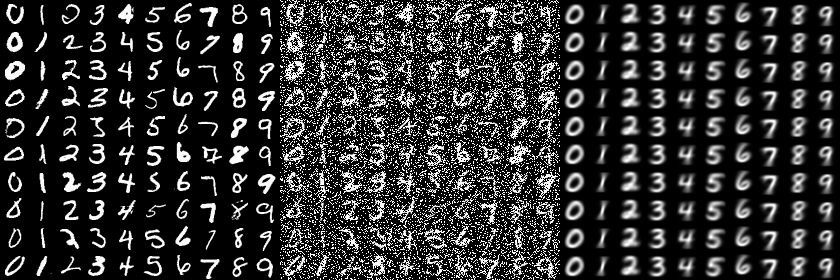
\includegraphics[width=0.5\textwidth]{s1}
\caption{RNN-GSN trained without noise scheduling on Sequence1 after 107 training epochs. Original sequence is on the left, noisy input to the model is in the middle, and output expected sequence is on the right.}\label{fig:s1}
\end{figure}

\textbf{Sequence2} introduces one bit of parity by alternating the sequences \{0,1,2,3,4,5,6,7,8,9,9,8,7,6,5,4,3,2,1,0...\} repeating, where the next value depends on whether the sequence is ascending or descending. The RNN-GSN is able to model this sequence as well, achieving a mean Parzen log-likelihood estimate of $-221.32 \pm 1.4$. The model was trained both with and without noise scheduling, and the outputs are compared in Figures \ref{fig:s2a} and \ref{fig:s2b}.
\begin{figure}[h!]
  \centering
    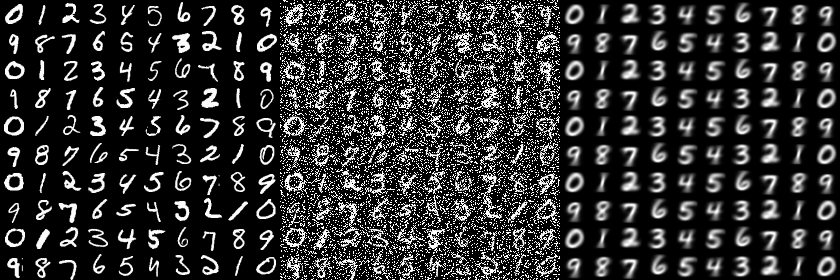
\includegraphics[width=0.5\textwidth]{s2a}
\caption{RNN-GSN trained without noise scheduling on Sequence2 after 132 training epochs. Original sequence is on the left, noisy input to the model is in the middle, and output expected sequence is on the right.}\label{fig:s2a}
\end{figure}
\begin{figure}[h!]
  \centering
    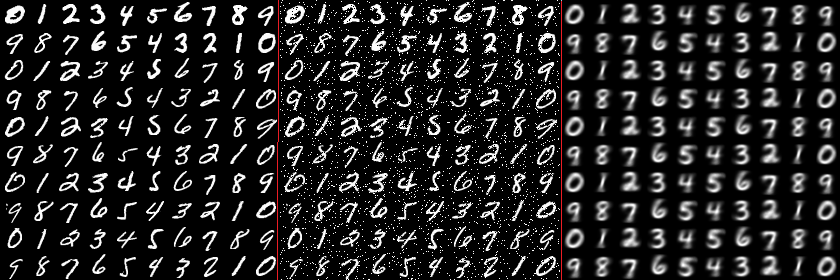
\includegraphics[width=0.5\textwidth]{s2b}
\caption{RNN-GSN trained with noise scheduling on Sequence2 after 115 training epochs. Original sequence is on the left, noisy input to the model is in the middle, and output expected sequence is on the right.}\label{fig:s2b}
\end{figure}


\textbf{Sequence3} creates a longer, more complex sequence by using multiple bits of parity. It is formed by Algorithm \ref{alg:s3}:
\begin{algorithm}
\caption{Sequence3}\label{alg:s3}
\begin{algorithmic}
	\STATE $sequence \Leftarrow [0,1,2]$
	\WHILE{not stop}
		\IF {$sequence[-3]$ is odd}
			\STATE $first\_bit = (sequence[-2] - sequence[-3])\%10$
		\ELSE
			\STATE $first\_bit = (sequence[-2] + sequence[-3])\%10$
		\ENDIF
		\IF {$first\_bit$ is odd}
			\STATE $second\_bit = (sequence[-1] - first\_bit)\%10$
		\ELSE
			\STATE $second\_bit = (sequence[-1] + first\_bit)\%10$
		\ENDIF
		\IF {$second\_bit$ is odd}
			\STATE $next\_num = (sequence[-1] - second\_bit)\%10$
		\ELSE
			\STATE $next\_num = (sequence[-1] + second\_bit)\%10$
		\ENDIF
		\STATE $sequence$ append $next\_num$
	\ENDWHILE
\end{algorithmic}
\end{algorithm}
This sequence has a length of 62 digits, which is longer than most conventional RNNs can learn without special techniques. As shown in Figure \ref{fig:s3}, the RNN-GSN can model the sequence fairly well and achieves a mean Parzen log-likelihood estimate of $-28.46 \pm 1.2$.
\begin{figure}[h!]
  \centering
    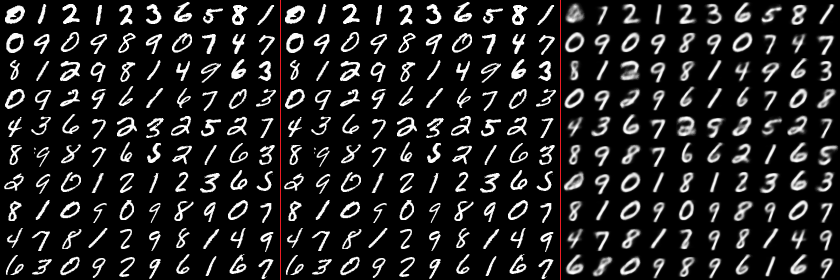
\includegraphics[width=0.5\textwidth]{s3}
\caption{RNN-GSN trained with noise scheduling on Sequence3 after 500 training epochs. Original sequence is on the left, noisy input to the model is in the middle, and output expected sequence is on the right.}\label{fig:s3}
\end{figure}

For reference, the Parzen estimate of a 2-layer, 4-walkback GSN trained on MNIST from \cite{gsn} is $-214 \pm 1.1$.

\subsection{Sequences of polyphonic music}
	We applied the RNN-GSN to probabilistic modeling of sequences of polyphonic music as MIDI files. Each dataset was used as described in \cite{rnnrbm}:

\textbf{Piano-midi.de} is a classical piano MIDI archive.\\
\textbf{Nottingham} is a collection of folk tunes.\\
\textbf{MuseData} is a library of orchestral and piano classical music from www.musedata.org.\\
\textbf{JSB chorales} is the corpus of 382 four-part harmonized chorales by J. S. Bach.
	
Log-likelihoods estimated by the Parzen density estimator are biased and cannot be compared to the AIS estimation used by Boulanger-Lewandowski et al. However, accuracies as computed by Bay et al. are provided for comparison \cite{bay}.

\begin {table}[H]
 \caption {MIDI accuracy \%} \label{tab:midi}
\begin{tabular}{l | l l l l}
\hline
Model & Piano-midi & Nottingham & Muse & JSB\\
\hline
RNN-RBM & 28.92 & 75.40 & 34.02 & 33.12\\
RNN-GSN  & xx.xx  & xx.xx  & xx.xx  & xx.xx\\
\hline
\end{tabular}
\end{table}

One important difference to note: the RNN-RBM uses the visible input $x$ when constructing the RBM for each timestep, and the RNN emits the bias parameters $b_h$ and $b_x$. Essentially, the RNN-RBM evaluates $P(X=x_t|H,b_t)$ for each timestep.

The RNN-GSN, on the other hand, only uses the hidden state $H_t$ emitted by the RNN to construct an expected input $\hat{x}_t$ for each timestep, sampling from the GSN's learned distribution $P(X|H)$. This means the predicted input at timestep $t$ is an expected value of the distribution $P(X|H_t)$. For a different accuracy measure, $P(X=x_t|H_t)$ could have been evaluated as well.